% ---* APENDICE *---
% Mostrar detalladamente el experimento de clustering (no técnico, eso va en implementacion)
% Tabla de las 5 mejores alternativas de clustering
% Grafico de todos contra todos
\chapter{Experimento de Clustering de Test}\aplabel{exp-clustering}

% Escribir el algoritmo original y el modificado

\par Para crear grupos de test a través del algoritmo de Agrupación Aglomerativo Jerárquico se necesita saber cuántos clusters se deben generar hacer que el algoritmo se detenga. Sin embargo a priori no se sabe cuántos se necesitan, pero sí se sabe que los clusters deben tener una similitud interna suficiente para que las comparaciones sean fructíferas y no una pérdida de tiempo. Para que esto pase, la similitud entre los par de tests debe ser de al menos un 80\%, por lo cual la similitud interna de cada cluster debe ser al menos de un 75\%. 
\par Además no se sabe tampoco qué medida de distancia entre clusters es la más apropiada para este problema: \emph{Single Link} (distancia entre los elementos más cercanos entre los dos clusters), \emph{Complete Link} (distancia entre los elementos más lejanos entre los dos clusters) o \emph{Average Link} (promedio entre todas las distancias de los pares que se pueden formar entre elementos de uno y otro cluster).  

\par Para determinar los mejores parámetros se realizó un experimento en el cual se ejecutó el algoritmo y en cada ejecución se varió la distancia ocupada y la similitud interna mínima que todos los clusters debían tener. Las tolerancias de similitud interna varíaron de la siguiente forma: 95\%, 90\%, 85\%, 80\% y 75\%.

\begin{figure}
\centering
\setlength{\tabcolsep}{1pt} % reducir la separacion entre columnas
\begin{tabular}[t]{cccc}
& \textbf{Single Link} & \textbf{Complete Link} & \textbf{Average Link} \\
% \textbf{95\%}
\subfloat{
\includegraphics[height=3.9cm]{images/clustering/95.pdf}}
   & \subfloat[45 Clusters]{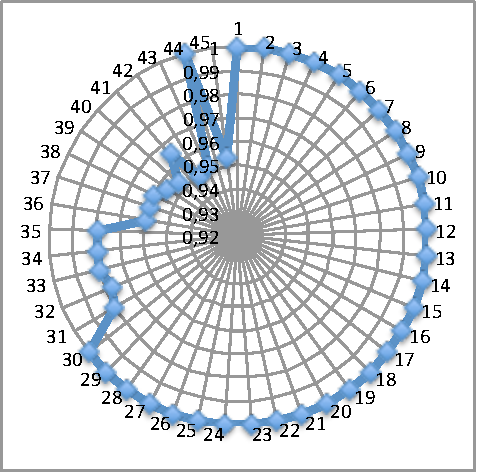
\includegraphics[width=3.9cm]{images/clustering/sl-95.pdf}} 
   & \subfloat[51 Clusters]{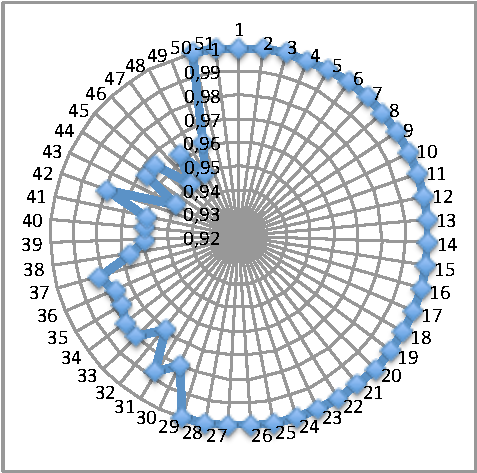
\includegraphics[width=3.9cm]{images/clustering/cl-95.pdf}}
   & \subfloat[47 Clusters]{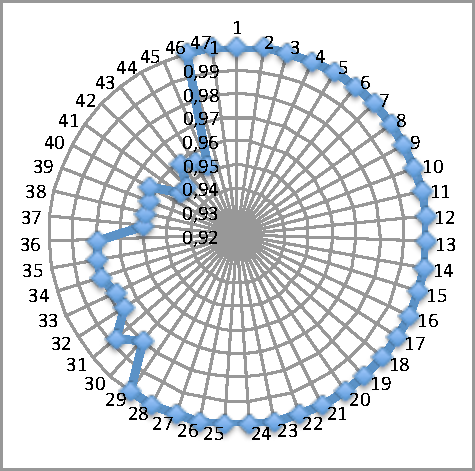
\includegraphics[width=3.9cm]{images/clustering/al-95.pdf}} \\[-0.1in] % reducir la separacion entre filas 

% \textbf{90\%}
\subfloat{
\includegraphics[height=3.9cm]{images/clustering/90.pdf}}
   & \subfloat[27 Clusters]{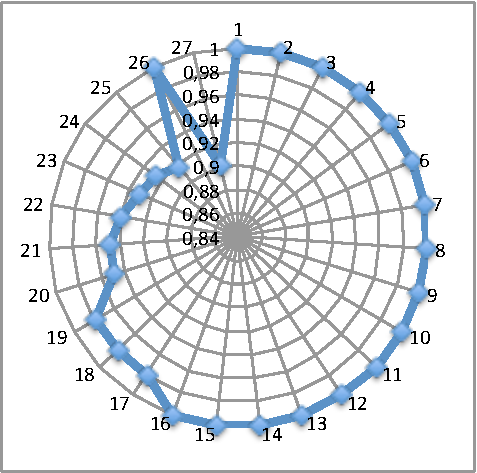
\includegraphics[width=3.9cm]{images/clustering/sl-90.pdf}} 
   & \subfloat[37 Clusters]{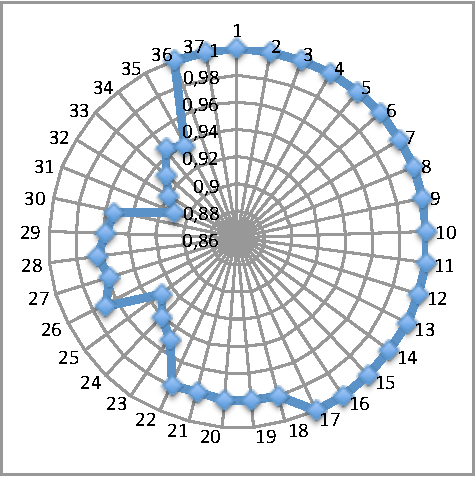
\includegraphics[width=3.9cm]{images/clustering/cl-90.pdf}}
   & \subfloat[29 Clusters]{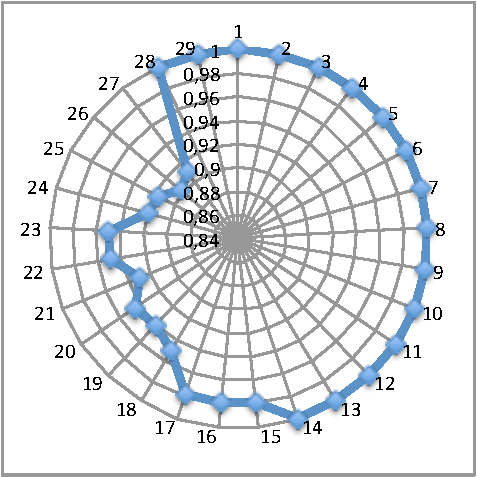
\includegraphics[width=3.9cm]{images/clustering/al-90.pdf}} \\[-0.1in]

% \textbf{85\%}
\subfloat{
\includegraphics[height=3.9cm]{images/clustering/85.pdf}}
   & \subfloat[22 Clusters]{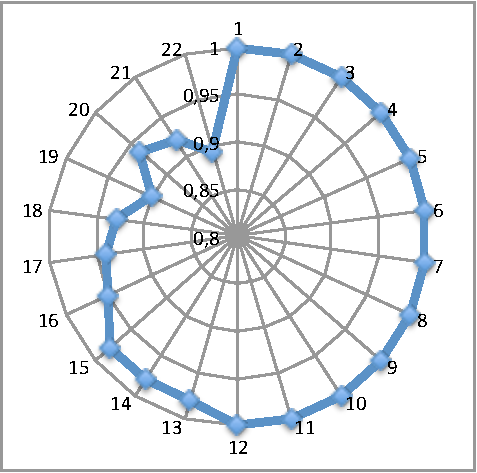
\includegraphics[width=3.9cm]{images/clustering/sl-85.pdf}} 
   & \subfloat[22 Clusters]{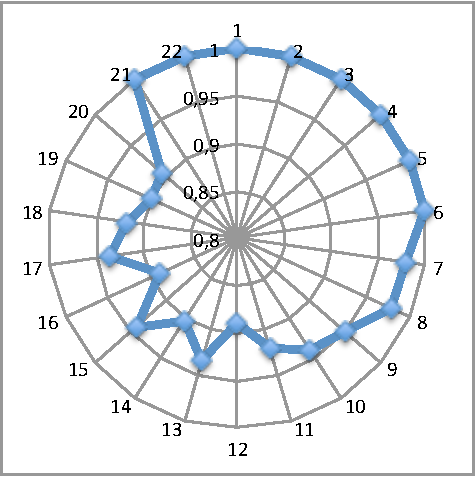
\includegraphics[width=3.9cm]{images/clustering/cl-85.pdf}}
   & \subfloat[20 Clusters]{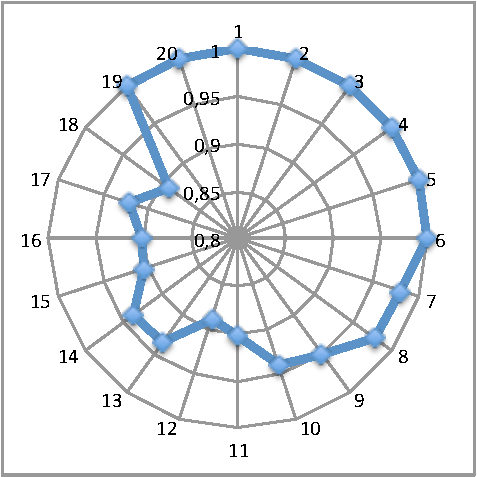
\includegraphics[width=3.9cm]{images/clustering/al-85.pdf}} \\[-0.1in]

% \textbf{80\%}
\subfloat{
\includegraphics[height=3.9cm]{images/clustering/80.pdf}}
   & \subfloat[13 Clusters]{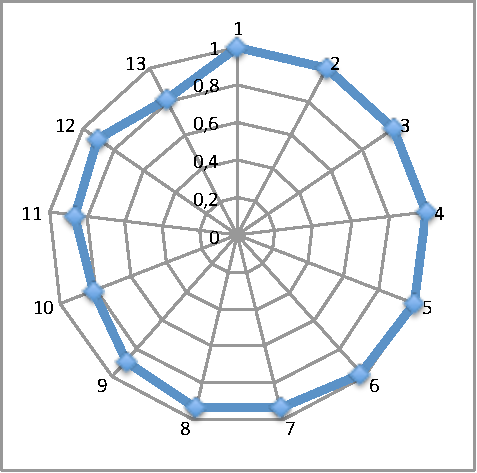
\includegraphics[width=3.9cm]{images/clustering/sl-80.pdf}} 
   & \subfloat[9 Clusters]{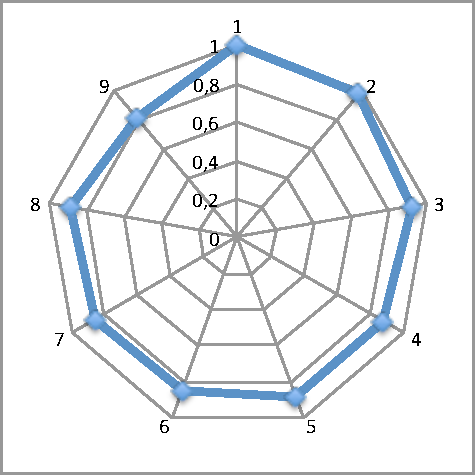
\includegraphics[width=3.9cm]{images/clustering/cl-80.pdf}}
   & \subfloat[7 Clusters]{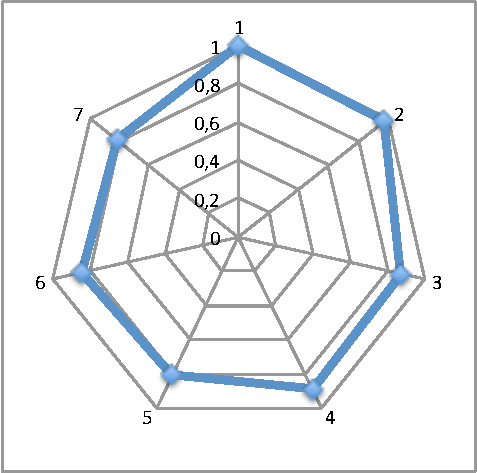
\includegraphics[width=3.9cm]{images/clustering/al-80.pdf}} \\[-0.1in]

% \textbf{75\%}
\subfloat{
\includegraphics[height=3.9cm]{images/clustering/75.pdf}}
   & \subfloat[9 Clusters]{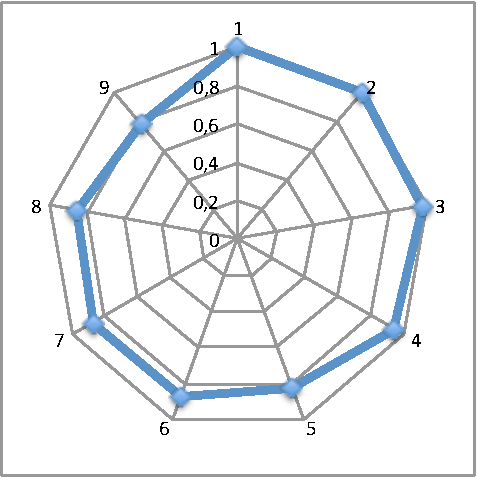
\includegraphics[width=3.9cm]{images/clustering/sl-75.pdf}} 
   & \subfloat[5 Clusters]{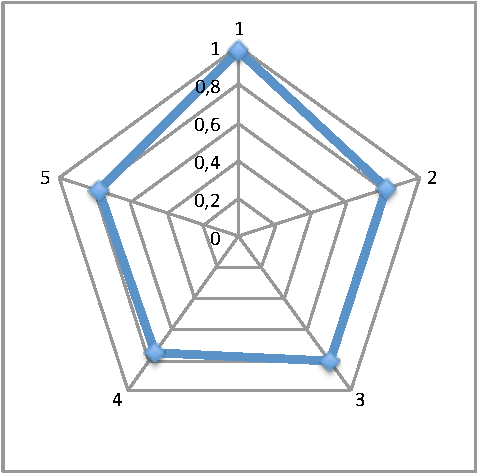
\includegraphics[width=3.9cm]{images/clustering/cl-75.pdf}}
   & \subfloat[5 Clusters]{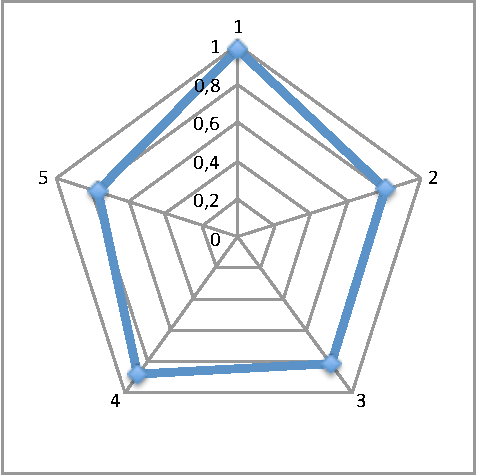
\includegraphics[width=3.9cm]{images/clustering/al-75.pdf}} \\[0in]    
\end{tabular}


\caption{Resultados experimento de Clustering de Tests por Similitud en Cobertura}\label{foo}
\end{figure}